\chapter{Lec 16 - Bayesian Learning II}

\section{Naive Bayes Classifier}
One of the simplest and most popular techniques based on Bayesian learning is the \textbf{Naive Bayes classifier}. It is an effective method when we have large data-sets and when the attributes describing the instances are conditionally independent given the classification.\newline\newline
Given a target function $f: X \rightarrow V$, with instances $x$ described by a set of attributes $\langle a_{1}, a_{2},...,a_{n}\rangle$, the most probable classification of a new instance $f(x)$ is:
\[v_{MAP} = argmax_{v_{j} \in V}P(v_{j} | a_{1}, a_{2},...,a_{n})\]
We want to maximize the probability to have class $v_{j}$ given the values of the instance attributes. By resorting to the Bayes formula, it follows that:
\[= argmax_{v_{j} \in V} \frac{P(a_{1}, a_{2},...,a_{n} | v_{j})P(v_{j})}{P(a_{1}, a_{2},...,a_{n})}\]
Note that $P(a_{1}, a_{2},...,a_{n})$ does not depend on $v_{j}$, so we can consider it as a constant and remove it from the formula:
\[= argmax_{v_{j} \in V} P(a_{1}, a_{2},...,a_{n} | v_{j})P(v_{j})\]
\begin{itemize}
    \item Compute $P(v_{j})$ is easy. We can compute the ratio between the occurrences of instances of class $v_{j}$ and the number of instances in the training set.

    \item Estimate $P(a_{1}, a_{2},...,a_{n} | v_{j})$ is \textbf{impossible}. This is because, since we should compute a probability for each combination of $a_{1}, a_{2},...,a_{n}$, which is computationally unfeasible. Furthermore, we need to see every  instance in the instance space many times in order to obtain reliable estimates. Hence, we would have a very, very large set of training data.
\end{itemize}
So, in order to overcome this problem, the Naive Bayes method makes an assumption:
\[P(a_{1}, a_{2},...,a_{n} | v_{j}) = \prod_{i}P(a_{i}|v_{j})\]
which means that the attributes describing an instance are independent each other.\newline\newline
Finally, the most probable class according to the Naive Bayes classifier is given by the following formula:
\[v_{NB} = argmax_{v_{j} \in V}P(v_{j})\prod_{i}P(a_{i}|v_{j})\]
One interesting difference between the naive Bayes learning method and other learning methods is that there is no explicit search through the space of possible hypotheses (in this case,  the  space of possible hypotheses is the space of possible values that can be assigned to the various $P(v_j)$ and $P(a_i|v_j)$ terms). Instead, the hypothesis is formed without searching, simply by counting the frequency of various data combinations within the training examples.

\subsection{Naive Bayes algorithm}
Given a training set $Tr$:
\begin{enumerate}
    \item For each target value $v_{j}$
    \begin{enumerate}
        \item $\hat{P}(v_{j}) \leftarrow$ estimate $P(v_{j})$ on $Tr$
        \item $\forall a_{i}$: $\hat{P}(a_{i} | v_{j}) \leftarrow$ estimate $P(a_{i} | v_{j})$ on $Tr$ (using the ratio method as done for $P(v_{j})$)
    \end{enumerate}
    \item return $\hat{P}(v_{j})$, $\hat{P}(a_{i} | v_{j})$ $\forall i,j$
\end{enumerate}
The \textbf{classification} of a new instance $x$ works as follows:
\begin{enumerate}
    \item $v_{NB} = argmax_{v_{j} \in V}\hat{P}(v_{j})\prod_{i}\hat{P}(a_{i}(x) | v_{j})$
    \item return $v_{NB}$
\end{enumerate}
where $a_{i}(x)$ is the value of the $i$-th attribute of the instance $x$.

\subsection{Naive Bayes: additional considerations}
The assumption of conditional independence is often violated, that is:
\[P(a_{1}, a_{2},...,a_{n}|v_{j}) \neq \prod_{i}P(a_{i}|v_{j})\]
Despite this, the Naive Bayes algorithm still works. This is because it is not necessary to correctly estimate the posterior probability $\hat{P}(v_{j}|x)$. It is sufficient that the order of those probability is \textit{correct}.\newline\newline
Note that if no training examples with target value $v_{j}$ has the attribute value $a_{i}$ equal to $k$, it follows that:
\[\hat{P}(a_{i} = k | v_{j}) = 0, \,\, and \,\, \hat{P}(v_{j})\prod_{i}\hat{P}(a_{i}|v_{j}) = 0\]
This can compromise the classification of the Naive Bayes method. A typical solution is the Bayesian \textit{m-estimate} for $\hat{P}(a_{i} | v_{j})$:
\[\hat{P}(a_{i} = k | v_{j}) \leftarrow \frac{n_{c} + mp_{k}}{n + m}\]
where:
\begin{itemize}
    \item $n$ is the number of training examples where $v = v_{j}$
    \item $n_{c}$ is the number of training examples where $v = v_{j}$ and $a = a_{i}$
    \item $p$ is the prior estimate of $\hat{P}(a_{i} | v_{j})$.
    \item $m$ is a constant which determines how heavily to weight $p$
\end{itemize}
Applications for Naive Bayes classifier are:
\begin{itemize}
    \item Diagnosis
    \item Classification of textual documents
\end{itemize}
In the context of text classification, it can be used to:
\begin{itemize}
    \item learn which documents are of interest
    \item learn to classify web pages by topic
    \item spam / no spam
    \item ...
\end{itemize}

\section{Learning to classify a text}
Given a document ($doc$), we want to classify it as interesting or not interesting for a particular user: $doc \rightarrow \{+, -\}$. We can represent a document by a vector of words where each word position in the document is an attribute:
\[doc = \{a_{1} = w_{1}, a_{2} = w_{2},..., a_{n} = w_{n}\}\]
We need to estimate the following probabilities:
\[P(+), \,\, P(-), \,\, P(doc | +), \,\, P(doc | -)\]
In this case, in addition to the assumption of conditional independence made before, we have to make another one:
\[P(a_{i} = w_{k} | v_{j}) = P(a_{m} = w_{k} | v_{j}), \,\, \forall i, j, k, m\]
where $P(a_{i} = w_{k} | v_{j})$ is the probability that the word in position $i$ is $w_{k}$, given $v_{j}$. Basically, we assume that the probability for each word to appear in any position is the same.\newline\newline
Therefore, we need to estimate \textit{only} the $P(v_{j}) \,\, \forall j$ and $P(w_{k} | v_{j}) \,\, \forall k, j$.\newline\newline
We can use a $m$-estimate with uniform priors and $m$ equal to the size of the vocabulary:
\[\hat{P}(w_{k} | v_{j}) = \frac{n_{k} + 1}{n + |Vocabulary|}\]
where
\begin{itemize}
    \item $n$ is the total number of word positions in all training documents having class $v_{j}$

    \item $n_{k}$ is the number of times the word $w_{k}$ is in these positions

    \item $|Vocabulary|$ is the total number of distinct words found in the training set.
\end{itemize}
\begin{center}
    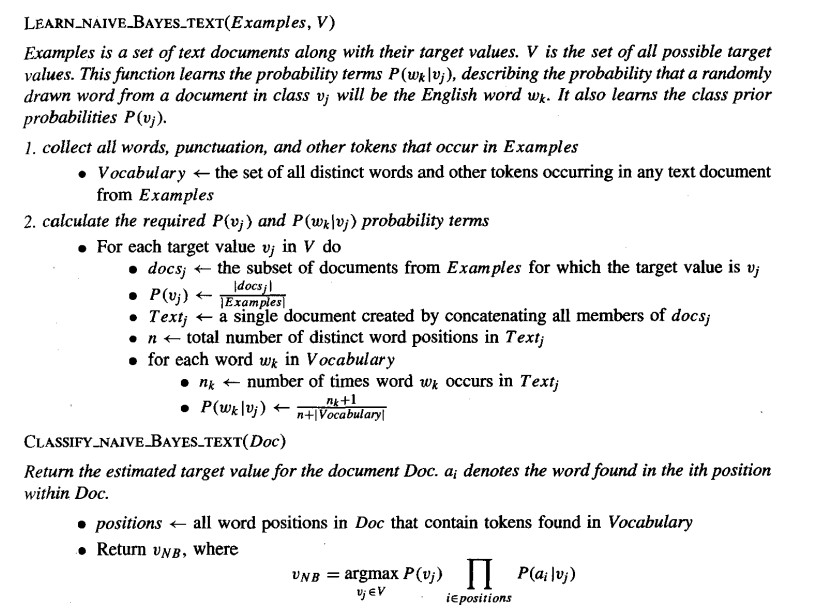
\includegraphics[]{images/training_naive_bayesian.png}
\end{center}

